\section{Nástěnný snímač prostorové teploty}

Pro snímání prostorové teploty z místností slouží nástěnný snímač prostorové teploty. Tyto zařízení primárně slouží k měření teploty a její následné odesílání do centrální jednotky. Disponují tlačítky pro nastavení požadované teploty (změna teploty s~krokem 0,5 °C) pro danou místnost. Aktuálně naměřenou a požadovanou teplotu zobrazují uživateli přímo na displeji. V případě přenastavení v~centrálním systému, dojde k propsání těchto změn přímo na jednotlivé snímací jednotky.  Nástěnný snímač prostorové teploty měří teplotu v místnosti každých 30~sekund. V~případě síťového výpadku komunikace se zařízení automaticky snaží připojení obnovit, samotný výpad je signalizován i~v~centrální jednotce. Jednotky existují ve dvou variantách. První varianta komunikace s centrální jednotkou pomocí Ethernetu a je napájena pomocí aktivního \acrshort{poe} (\textit{\acrlong{poe}}). Druhá varianta komunikuje s centrální jednotkou pomocí bezdrátové sítě WiFi a je napájena pomocí síťového adaptéru. Obě varianty jsou popsány níže v sekci \ref{sec:ethernet-modul} a \ref{sec:wifi-modul}. Celkově je po domě umístěno 6 zařízení s Ethernetem a~4 zařízení s WiFi. DPS byly vlastnoručně navrženy, pro výrobu byla použita firma JLCPCB \cite{jlcpcb}, součástky byly vlastnoručně osazeny.

\subsection{Varianta s Ethernetem}
\label{sec:ethernet-modul}

\begin{figure}[H]
   \centering
   \def\svgwidth{0.5\columnwidth}
   \input{images/svg/otopna-soustava/vyrez-nastenny-snimac-prostorove-teploty-ethernet.pdf_tex}
    \caption[Výřez pro umístění nástěnných snímačů prostorové teploty (verze Ethernet).]{Výřez z obrázku \ref{fig:otopna-soustava-a-elektronika-rez-domu} – umístění nástěnných snímačů prostorové teploty (verze Ethernet).}
    \label{fig:vyrez-nastenny-snimac-prostorove-teploty-ethernet}
\end{figure}

Na obrázku \ref{fig:vyrez-nastenny-snimac-prostorove-teploty-ethernet} je výřez části z celkového nákresu (obrázek \ref{fig:otopna-soustava-a-elektronika-rez-domu}) pro nástěnné snímače prostorové teploty (verze Ethernet). Na obrázku \ref{fig:blokove-schema-nastenny-snimac-teploty-ethernet} je blokové schéma nástěnného snímače prostorové teploty komunikující pomocí Ethernetu a je napájen pomocí aktivního POE. Snímač je napájen ze zařízení \acrshort{pse} (\textit{\acrlong{pse}}) (jedná se o POE switch MaxLink PSAT-10-8P-250 \cite{maxlink-psat-10-8p-250}), které řídí vykomunikování napájení a~výkonnostní třídy pro koncové zařízení (snímač (\acrshort{pd} (\textit{\acrlong{pd}}))). Jak zařízení PSE, tak PD podporují standart 802.3af \cite{norma-802.3af} respektive 802.3at \cite{norma-802.3at}. Zařízení PD jsou nastavená pro nejnižší definovanou výkonovou třídu 1 (max. výkon PSE pro jednotlivé PD zařízení je 4 W). Pro přenos napětí se využívají tzv. fantomové napětí, kdy v případě využití páru 1,2 a 3,6 se stejnosměrné napětí vyvede ze středu transformátoru. Další možností je využití volných párů 4,5 a 7,8 (zejména při rychlosti 10 nebo 100~Mbit/s (využity pro přenos dat 2 páry)). Vstupní napětí z PSE (44–57 V v~závislosti na délce kabelu UTP a~ztrátách) prochází přes diodový usměrňovač (nezávislost kladného pólu zdroje a země). Je zde řídící obvod TPS23753A \cite{tps23753a}, který zajišťuje komunikaci/rozhraní pro správné nastavení a povolení napětí z PSE, dále zajišťuje řízení převodu vstupního napětí na výstupní napětí 5~V (DC-DC měnič), je zapojen v~topologie Flyback (využívá tedy vázaný induktor). Zpětná vazba je řešena pomocí optické zpětné vazby s nastavitelnou Zenerovou diodou TLV431A \cite{tlv431a} v~zapojení komparátoru. Při návrhu zdrojové části zařízení bylo vycházelo z referenčního návrhu od výrobce Texas Instruments pro integrovaný obvod TPS23753A.

Zařízení v provozu je primárně  napájeno pomocí 5 V, v případě programování zařízení je možné použít programovací konektor s napájecím pinem pro 5 V. Pokud je k~dispozici POE, dojde zablokování napájení z programovacího konektoru (pomocí MOSFETu s~kanálem P). Napětí 5~V je následně vedeno do dvou \acrshort{ldo} (\textit{\acrlong{ldo}}) regulátorů. Jeden slouží pouze pro napájení ESP-32-WROVER-IE (M213EH2864UH3Q0) \cite{esp32-wrover-ie} modulu, druhý je pro napájení zbylých periferií (displej, tlačítka, teplotní senzor, obvod pro fyzickou vrstvu Ethernetu W5500 \cite{w5500}). Důvodem rozdělení je proudové rozdělení jednotlivých regulátorů a tedy i jejich ztrátové teplo. Vzhledem k~parametrům udávané výrobcem modulu ESP32 je možné max. proudový odběr až 0,5~A (proto byl vybrán regulátor, který toto zatížení dlouhodobě zvládne při daném úbytku napětí i když se reálně nepředpokládá, že k tomuto zatížení dojde). Dále bylo zohledněno, pokud by došlo k~ESD události (jedná se o~zařízení na které uživatelé sahají), tak je žádoucí, aby došlo maximálně k~restartu periferií a ne k restartu samotného ESP32 modulu. 

Pro programování modulu je zde konektor pro připojení externího modulu (viz část \ref{sec:prevodnik-usb-uart-cp2102n}), kde jsou piny pro TX/RX signál z UART a signály na automatický reset a boot modulu a piny pro napájení 5 V a země. Dále jsou zde přímo na DPS umístěná tlačítka pro boot a reset ESP32 modulu bez závislosti připojení programovacího modulu (lze tedy programovat i jinými moduly, které nemají automatický reset a boot). 

Samotné zařízení disponujeme ohranými transily na místech konektorů a~částí, které jsou přímo v kontaktu s uživatelem. Samotný obvod pro POE též disponuje proudovou a teplotní ochranou. LDO regulátory disponují detekcí nízkého vstupního napětí pro úspěšné spuštění, teplotní pojistkou a ochranou při zvýšení výstupního napětí vůči vstupnímu. 

Pro zobrazování aktuální a požadované teploty je barevný TFT displej velikosti 2.2" (240×320 pixelů) s řadičem ILI9341 \cite{lcd-ili9341}. Displej je připojen k~ESP32 modulu pomocí SPI sběrnice. Displej disponuje možností ovládání podsvícení pomocí PWM. Pro fyzickou vrstvu slouží obvod W5500, který implementuje ethernetový řadič s integrovaným TCP/IP. Obvod je s modulem ESP32 připojen pomocí SPI sběrnice. Pro snímání teploty slouží teplotní senzor DS18B20 (viz sekce \ref{sec:teplotni-senzory}). V neposlední řadě jsou zde tři tlačítka pro nastavení požadované teploty a~vyvolání nabídky menu.

Modul ESP32 disponuje rozhraním \acrshort{rmii} (\textit{\acrlong{rmii}}), který má složitější softwarovou implementaci a využívá větší počet pinů. Proto je zvolen integrovaný obvod W5500. Použití i využití následných knihoven bylo mnohem jednodušší. Vzhledem k malému vytížení komunikace je tento obvod dostačující. Pro komunikace mezi modulem ESP32 a displejem a obvodem W5500 jsou využity dvě nezávislé SPI sběrnice. 

V příloze \ref{app:nastenny-snimac-prostorove-teploty-ethernet} je schéma snímací jednotky. Na obrázku \ref{fig:dps-nastenny-snimac-prostorove-teploty-ethernet-vrchni-cast} je vrchní část realizované DPS pro snímací jednotku. Pro lepší galvanické oddělení jsou vyfrézované drážky. Dále na obrázku \ref{fig:dps-nastenny-snimac-prostorove-teploty-ethernet-vrchni-cast-displej} je DPS s osazeným displejem. Na obrázku \ref{fig:dps-nastenny-snimac-prostorove-teploty-ethernet-spodni-cast} je spodní část DPS. Kompletní zařízení včetně umístění do krabičky a popis samotné krabičky je v části \ref{sec:krabicka-pro-nastenny-snimac-prostorove-teploty}.



\begin{figure}[H]
    \centering
    \def\svgwidth{\columnwidth}
    \input{images/svg/blokove-schema-nastenny-snimac-teploty-ethernet.pdf_tex}
    \caption[]{Blokové schéma nástěnného snímače prostorové teploty (verze Ethernet).}
    \label{fig:blokove-schema-nastenny-snimac-teploty-ethernet}
\end{figure}


\begin{figure}[H]
\centering
\begin{subfigure}{.5\textwidth}
  \centering
  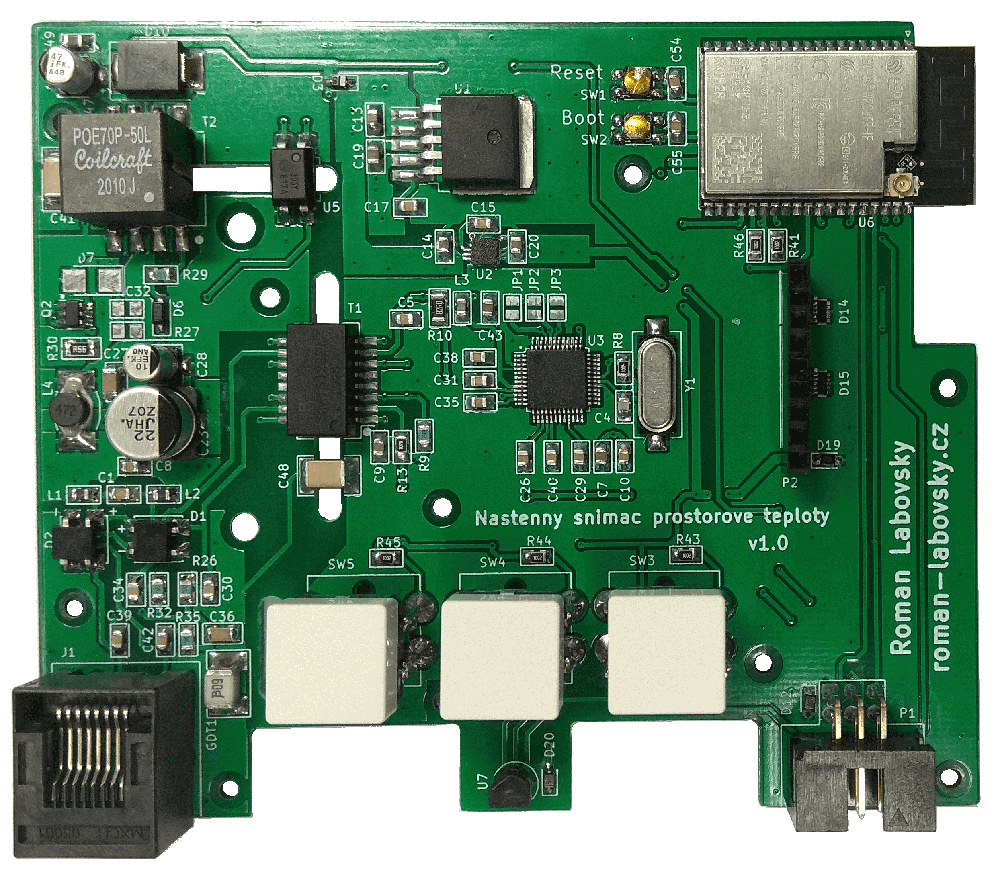
\includegraphics[width=\textwidth]{images/nastenny-snimac-prostorove-teploty-ethernet/dps-nastenny-snimac-prostorove-teploty-ethernet-vrchni-cast.png}
  \caption{Vrchní strana.}
  \label{fig:dps-nastenny-snimac-prostorove-teploty-ethernet-vrchni-cast}
\end{subfigure}%
\begin{subfigure}{.5\textwidth}
  \centering
  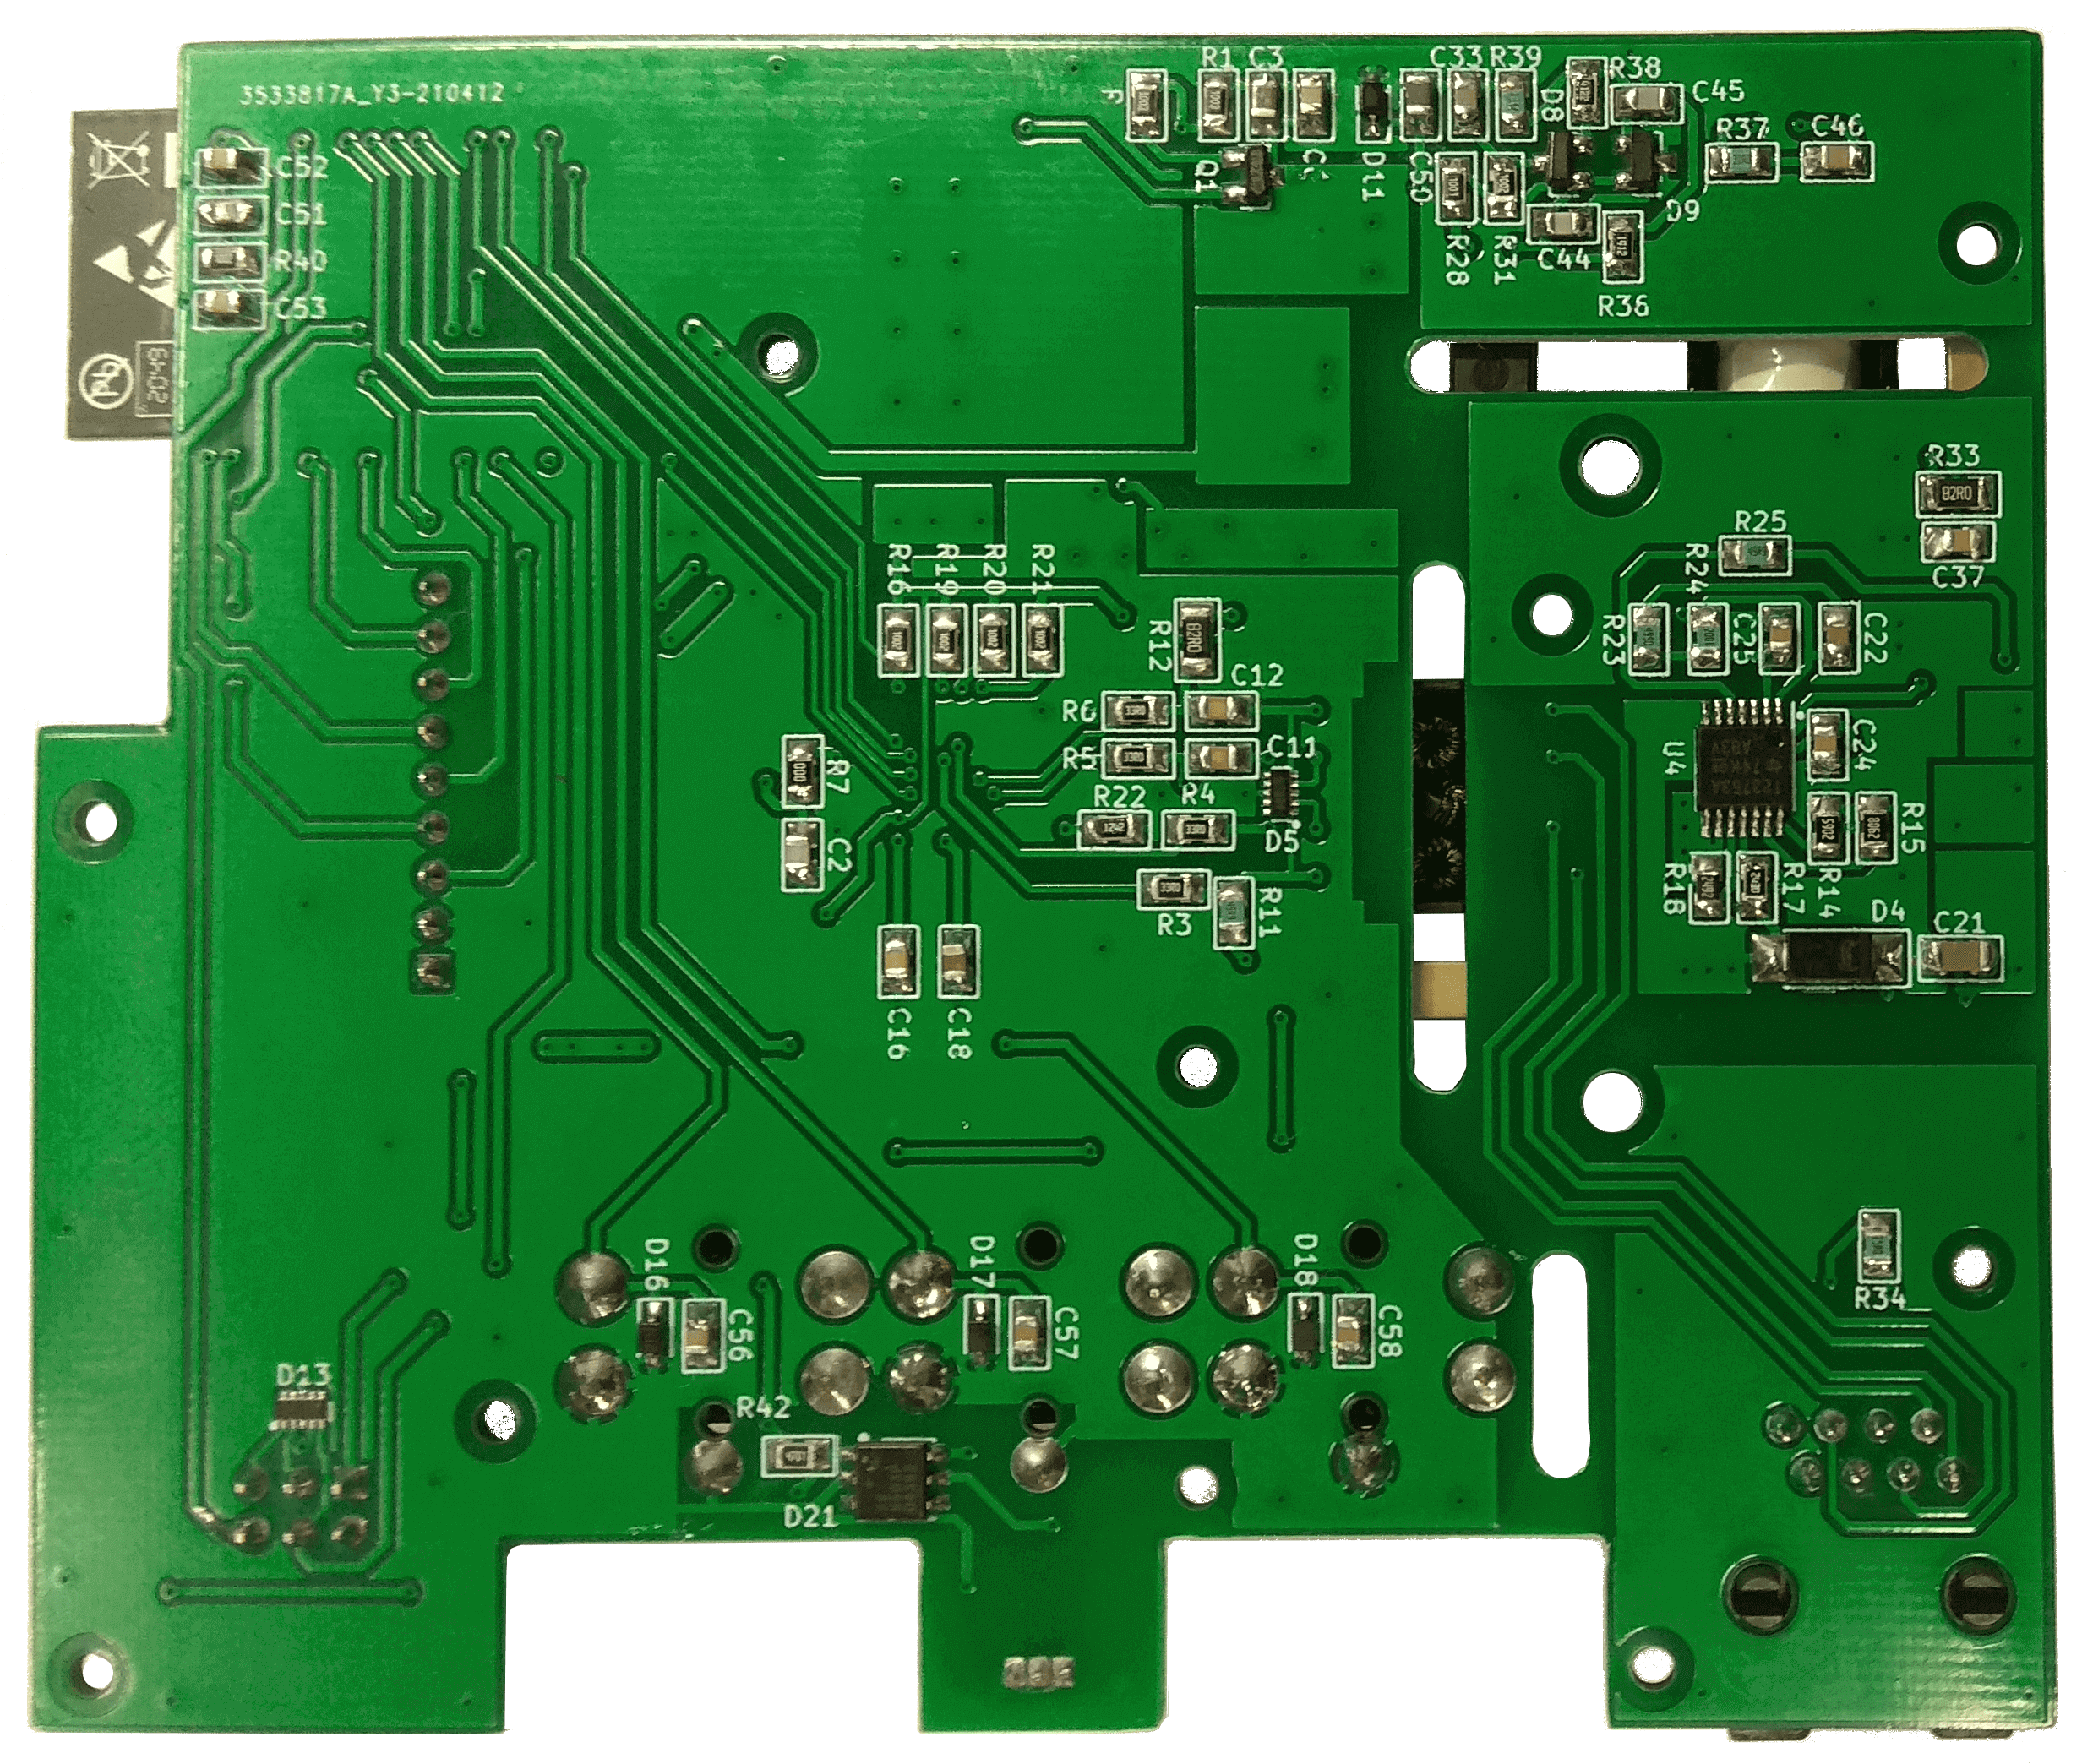
\includegraphics[width=\textwidth]{images/nastenny-snimac-prostorove-teploty-ethernet/dps-nastenny-snimac-prostorove-teploty-ethernet-spodni-cast.png}
  \caption{Spodní strana.}
  \label{fig:dps-nastenny-snimac-prostorove-teploty-ethernet-spodni-cast}
\end{subfigure}
\caption{DPS nástěnného snímače prostorové teploty (verze Ethernet).}
\label{fig:dps-nastenny-snimac-prostorove-teploty-ethernet}
\end{figure}


\begin{figure}[H]
    \centering
    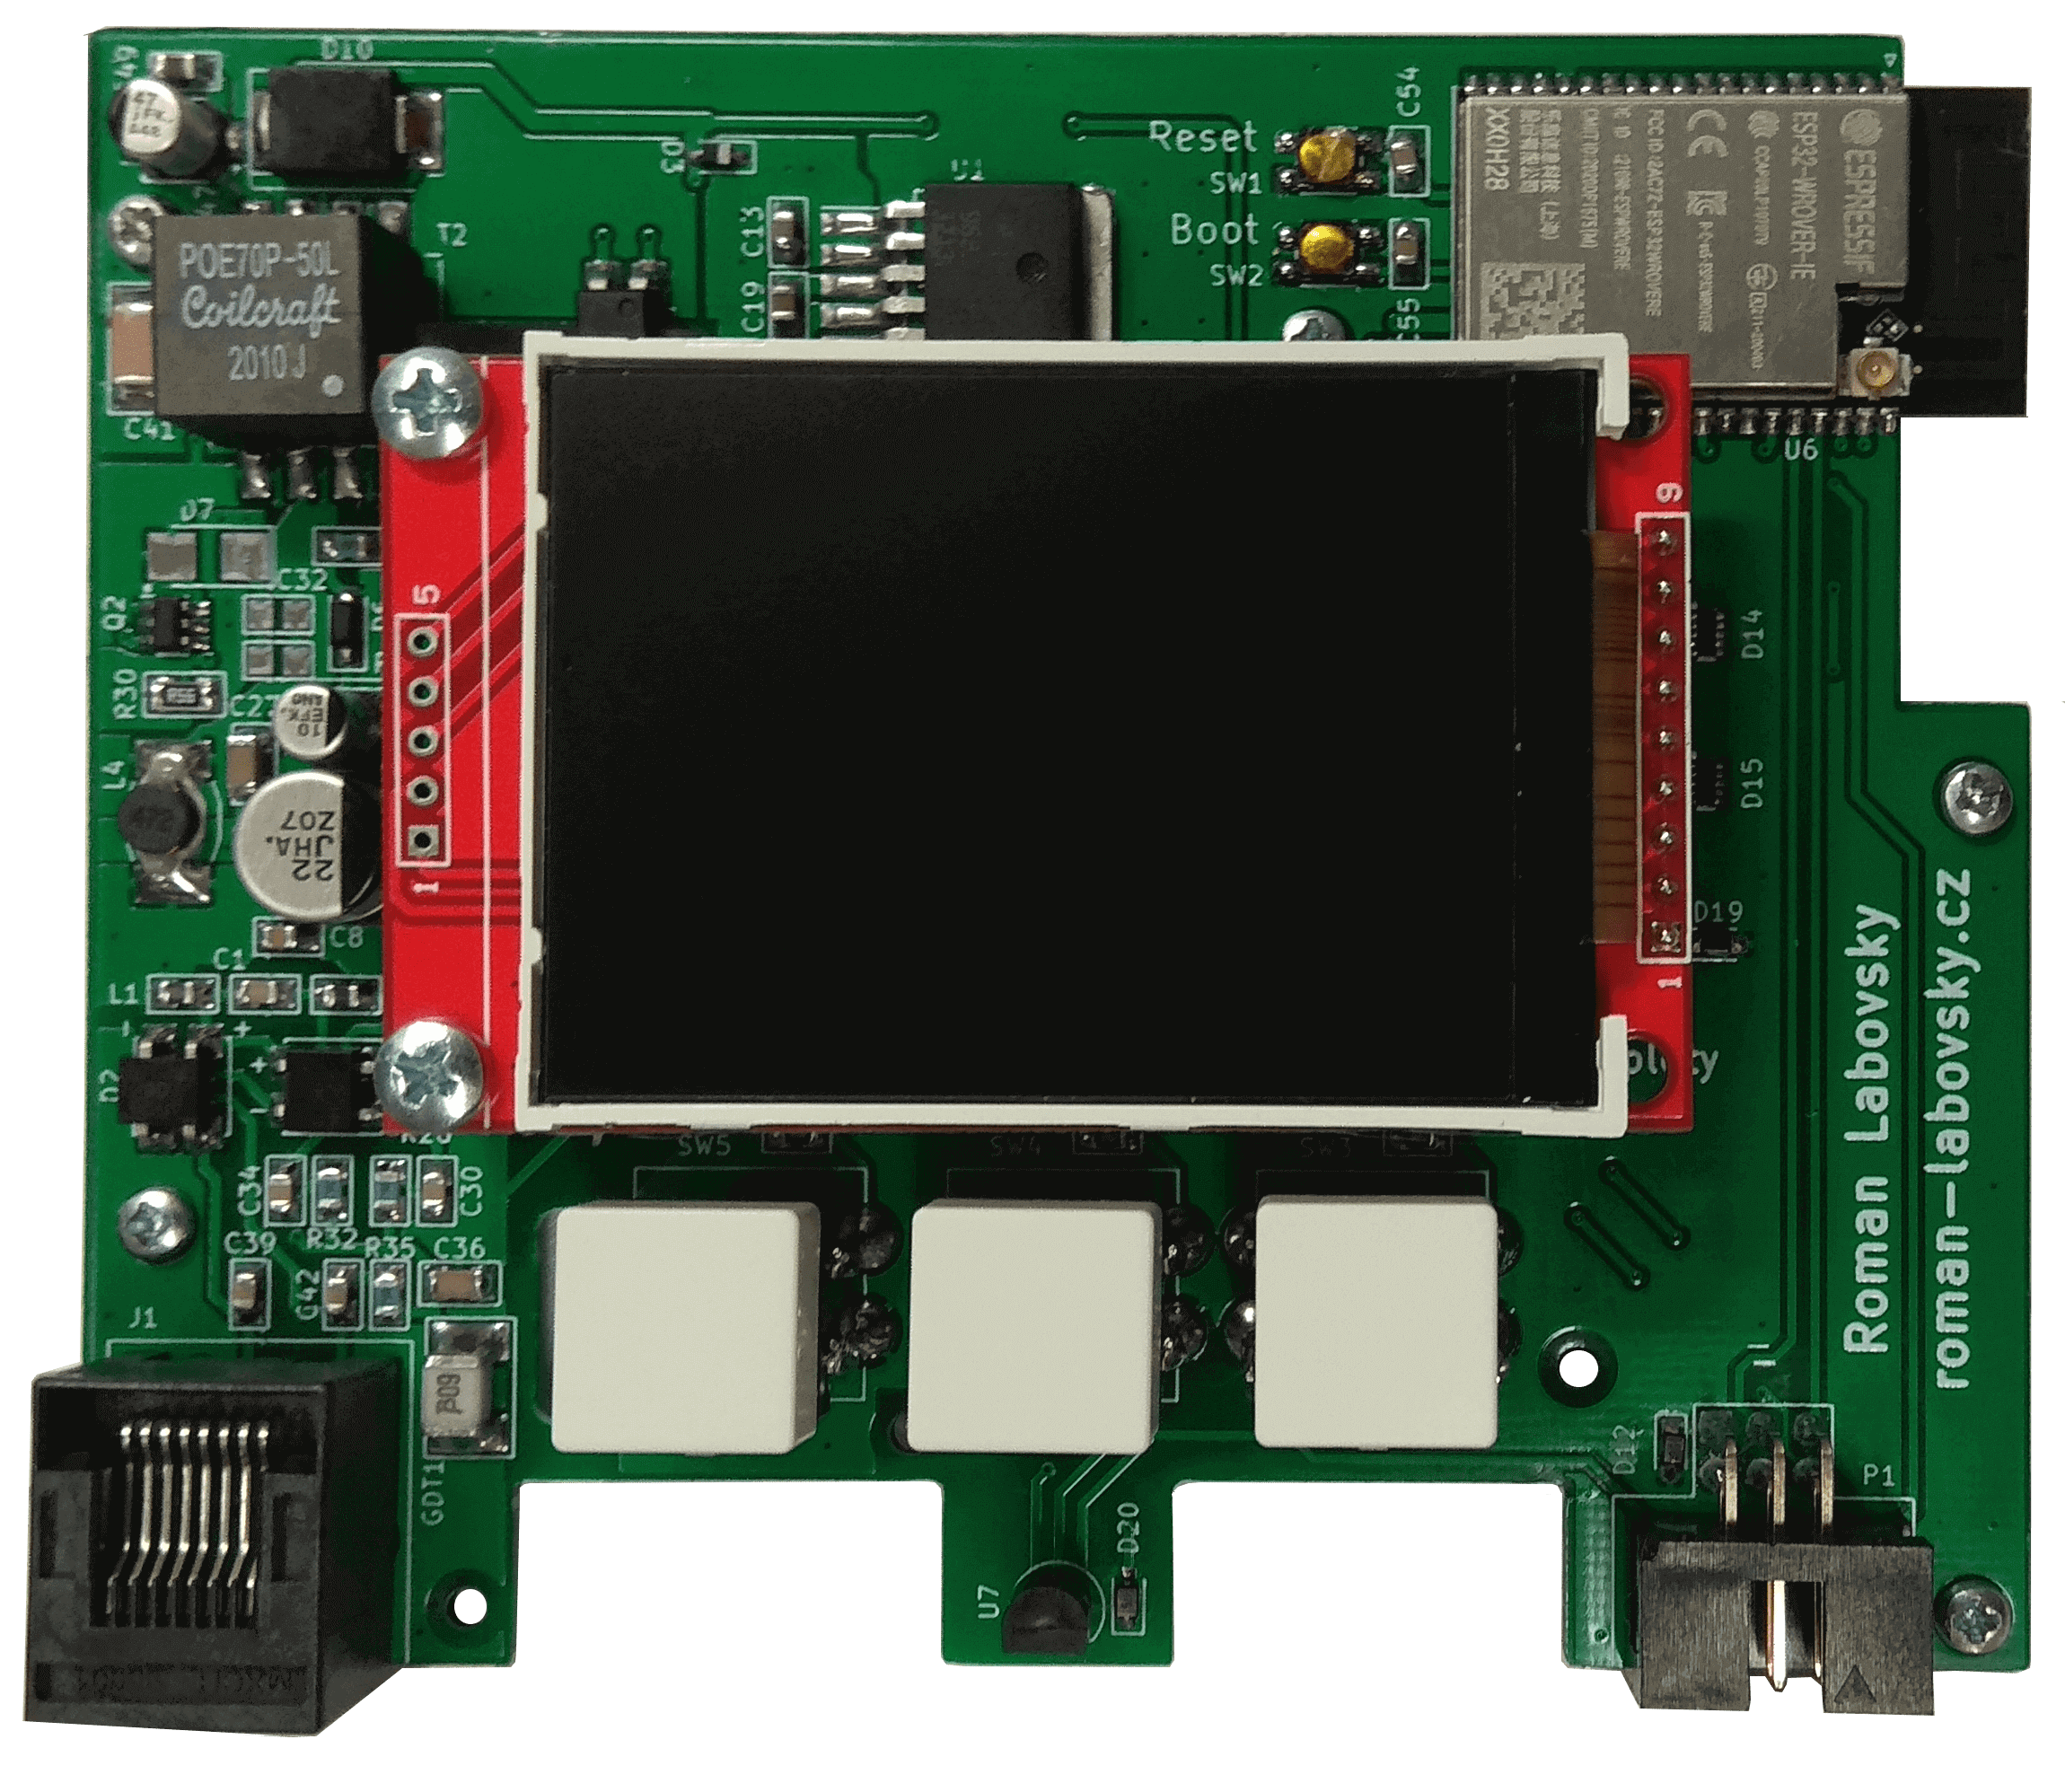
\includegraphics[width=0.88\textwidth]{images/nastenny-snimac-prostorove-teploty-ethernet/dps-nastenny-snimac-prostorove-teploty-ethernet-vrchni-cast-displej.png}
    \caption{DPS nástěnného snímače prostorové teploty (verze Ethernet) s~displejem, vrchní strana.}
    \label{fig:dps-nastenny-snimac-prostorove-teploty-ethernet-vrchni-cast-displej}
\end{figure}



\subsection{Varianta s WiFi}
\label{sec:wifi-modul}


\begin{figure}[H]
   \centering
   \def\svgwidth{0.5\columnwidth}
   \input{images/svg/otopna-soustava/vyrez-nastenny-snimac-prostorove-teploty-wifi.pdf_tex}
    \caption[Výřez umístění nástěnných snímačů prostorové teploty (verze WiFi).]{Výřez z obrázku \ref{fig:otopna-soustava-a-elektronika-rez-domu} – umístění nástěnných snímačů prostorové teploty (verze WiFi).}
    \label{fig:vyrez-nastenny-snimac-prostorove-teploty-wifi}
\end{figure}

Na obrázku \ref{fig:vyrez-nastenny-snimac-prostorove-teploty-wifi} je výřez části z celkového nákresu (obrázek \ref{fig:otopna-soustava-a-elektronika-rez-domu}) systému znázorňující umístění nástěnných snímačů prostorové teploty (verze WiFi). Na obrázku \ref{fig:blokove-schema-nastenny-snimac-teploty-wifi} je blokové schéma nástěnného snímače prostorové teploty komunikující pomocí WiFi a je napájen pomocí síťového adaptéru (Mean Well GSM06E05-P1J \cite{gsm06e05-p1j}). Oproti verzi z \ref{sec:ethernet-modul} chybí celá část tykající se POE napájení a~také obvod W5500 implementující ethernetovou komunikaci. Zbylé části jsou totožné jako v části \ref{sec:ethernet-modul}.

V příloze \ref{app:nastenny-snimac-prostorove-teploty-wifi} je schéma snímací jednotky. Na obrázku \ref{fig:dps-nastenny-snimac-prostorove-teploty-wifi-vrchni-cast} je vrchní část realizované DPS pro snímací jednotku. Dále na obrázku \ref{fig:dps-nastenny-snimac-prostorove-teploty-wifi-vrchni-cast-displej} je DPS s osazeným displejem. Na obrázku \ref{fig:dps-nastenny-snimac-prostorove-teploty-wifi-spodni-cast} je spodní část DPS. Kompletní zařízení včetně umístění do krabičky a popis samotné krabičky je v části \ref{sec:krabicka-pro-nastenny-snimac-prostorove-teploty}.

\begin{figure}[H]
    \centering
    \def\svgwidth{\columnwidth}
    \input{images/svg/blokove-schema-nastenny-snimac-teploty-wifi.pdf_tex}
    \caption[]{Blokové schéma nástěnného snímače prostorové teploty (verze WiFi).}
    \label{fig:blokove-schema-nastenny-snimac-teploty-wifi}
\end{figure}


\begin{figure}[H]
\centering
\begin{subfigure}{.5\textwidth}
  \centering
    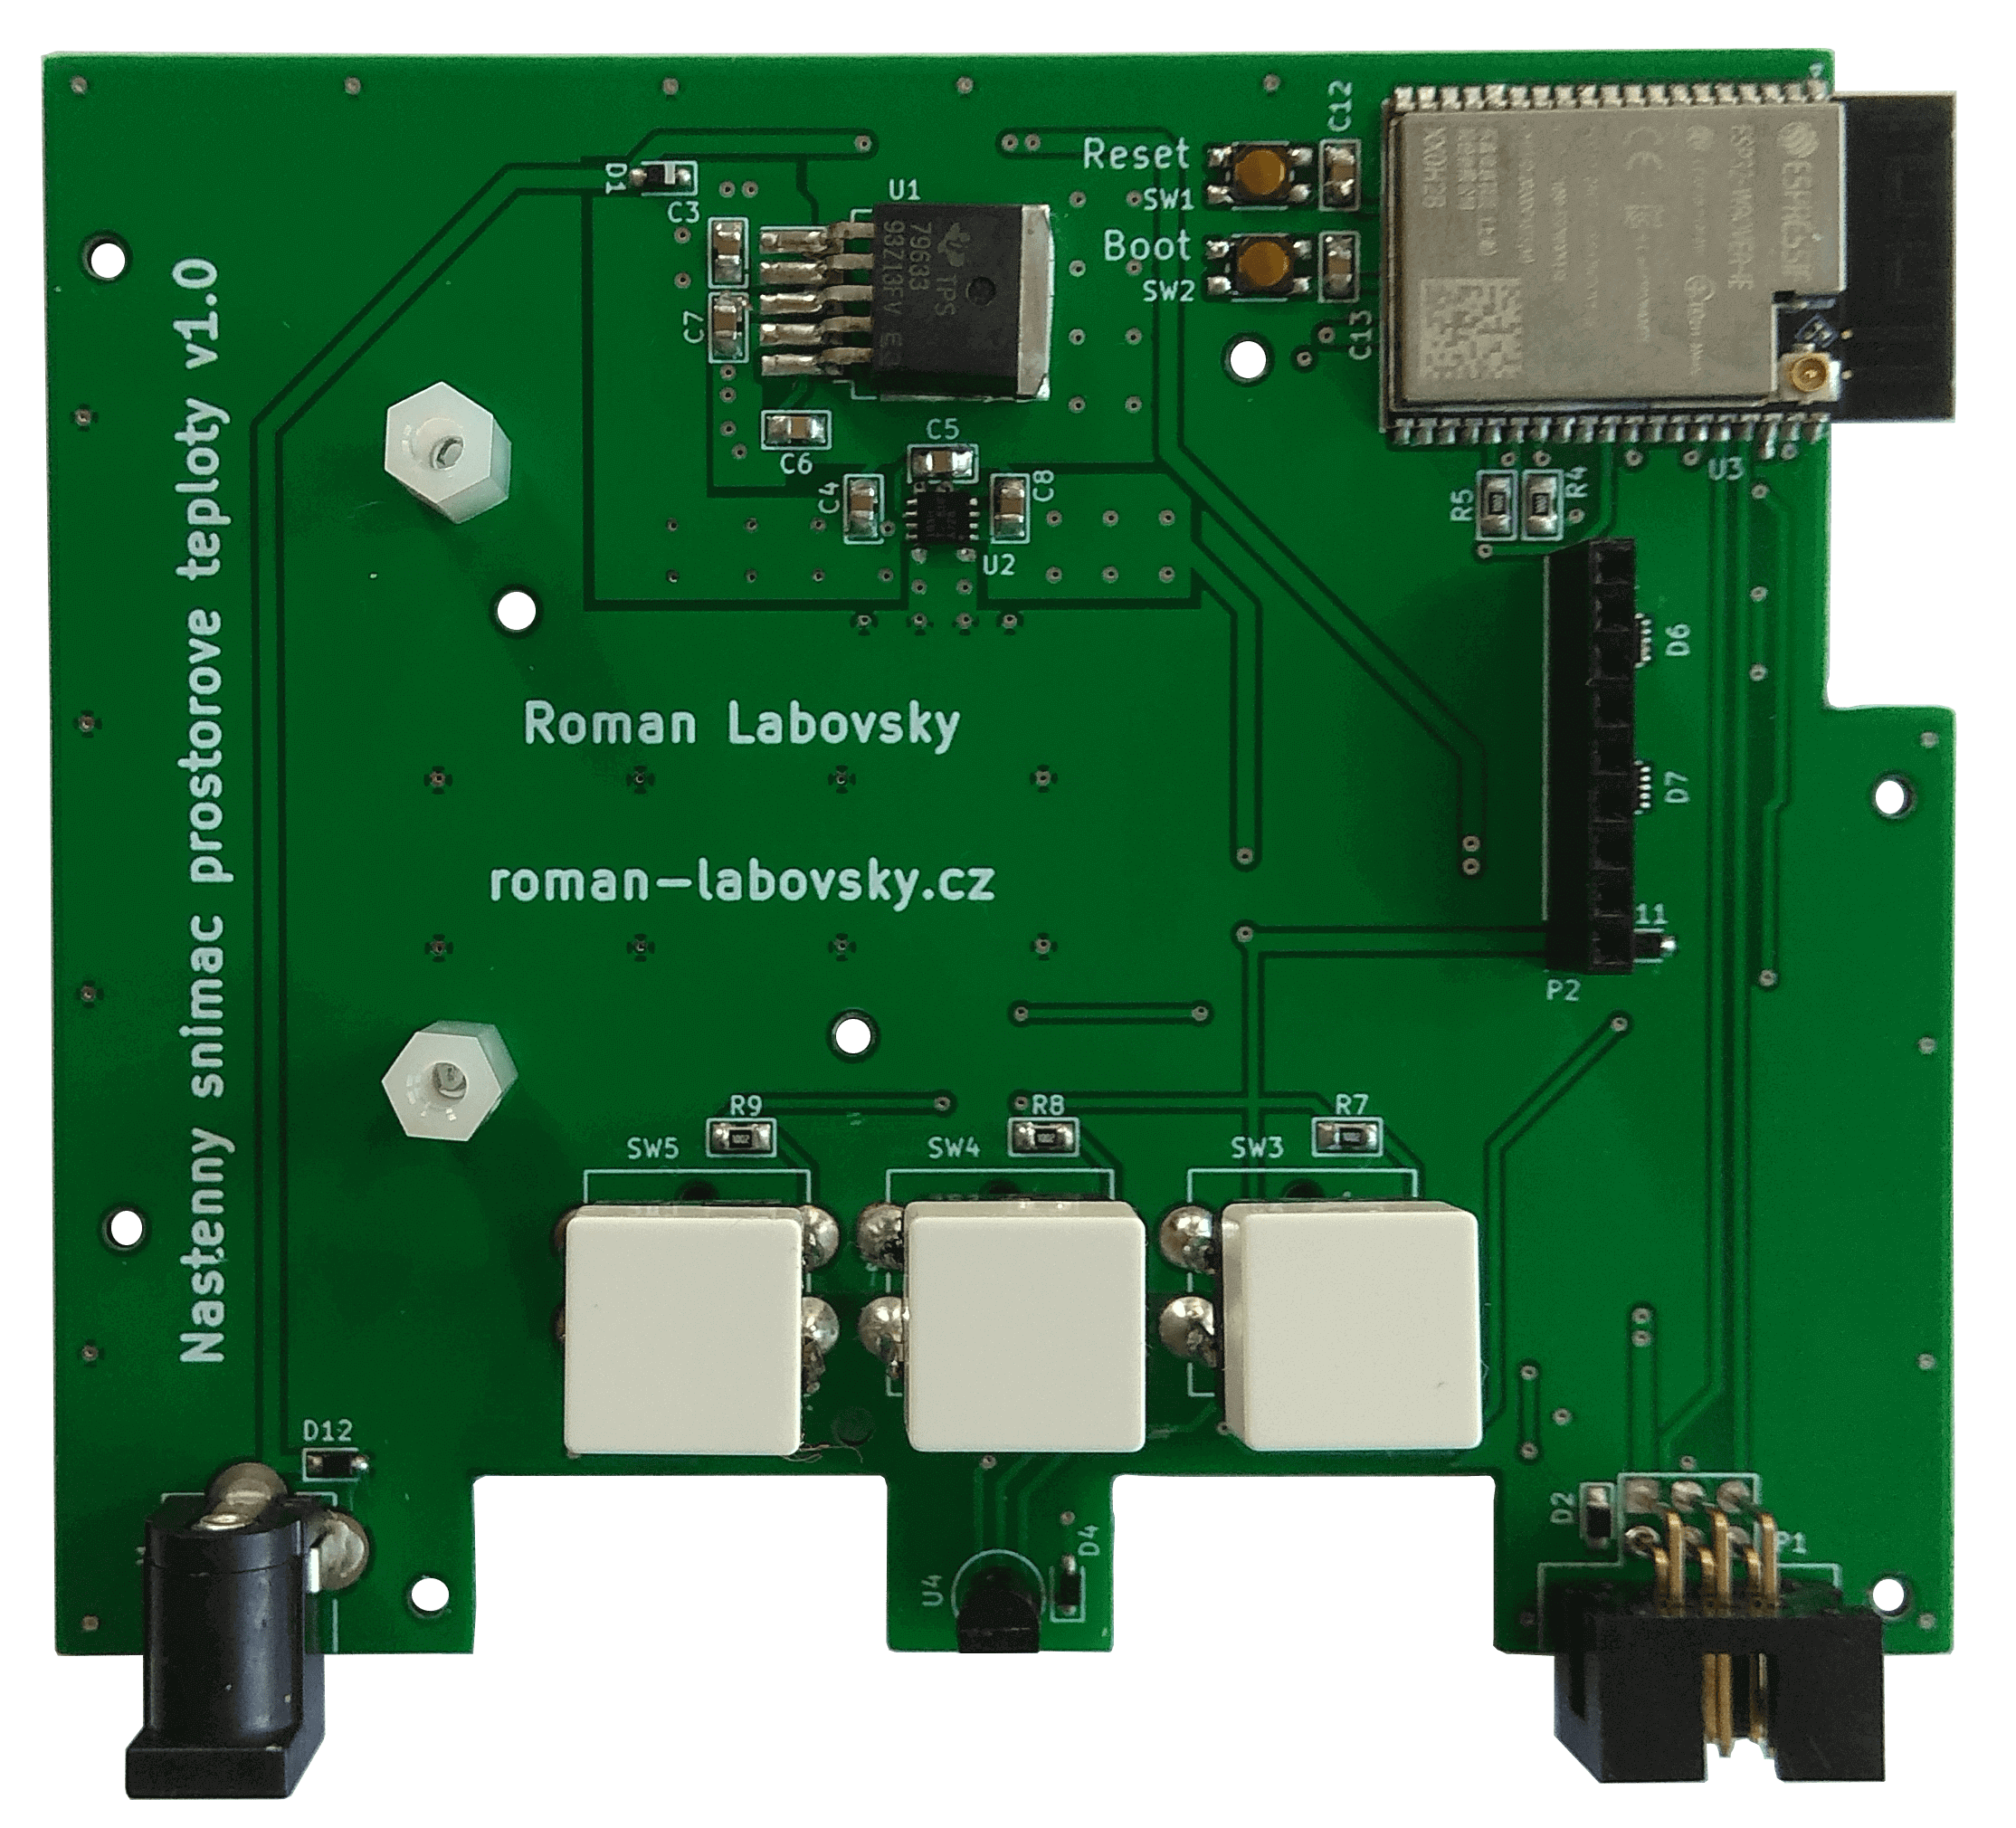
\includegraphics[width=\textwidth]{images/nastenny-snimac-prostorove-teploty-wifi/dps-nastenny-snimac-prostorove-teploty-wifi-vrchni-cast.png}
    \caption{Vrchní strana.}
    \label{fig:dps-nastenny-snimac-prostorove-teploty-wifi-vrchni-cast}
\end{subfigure}%
\begin{subfigure}{.5\textwidth}
  \centering
    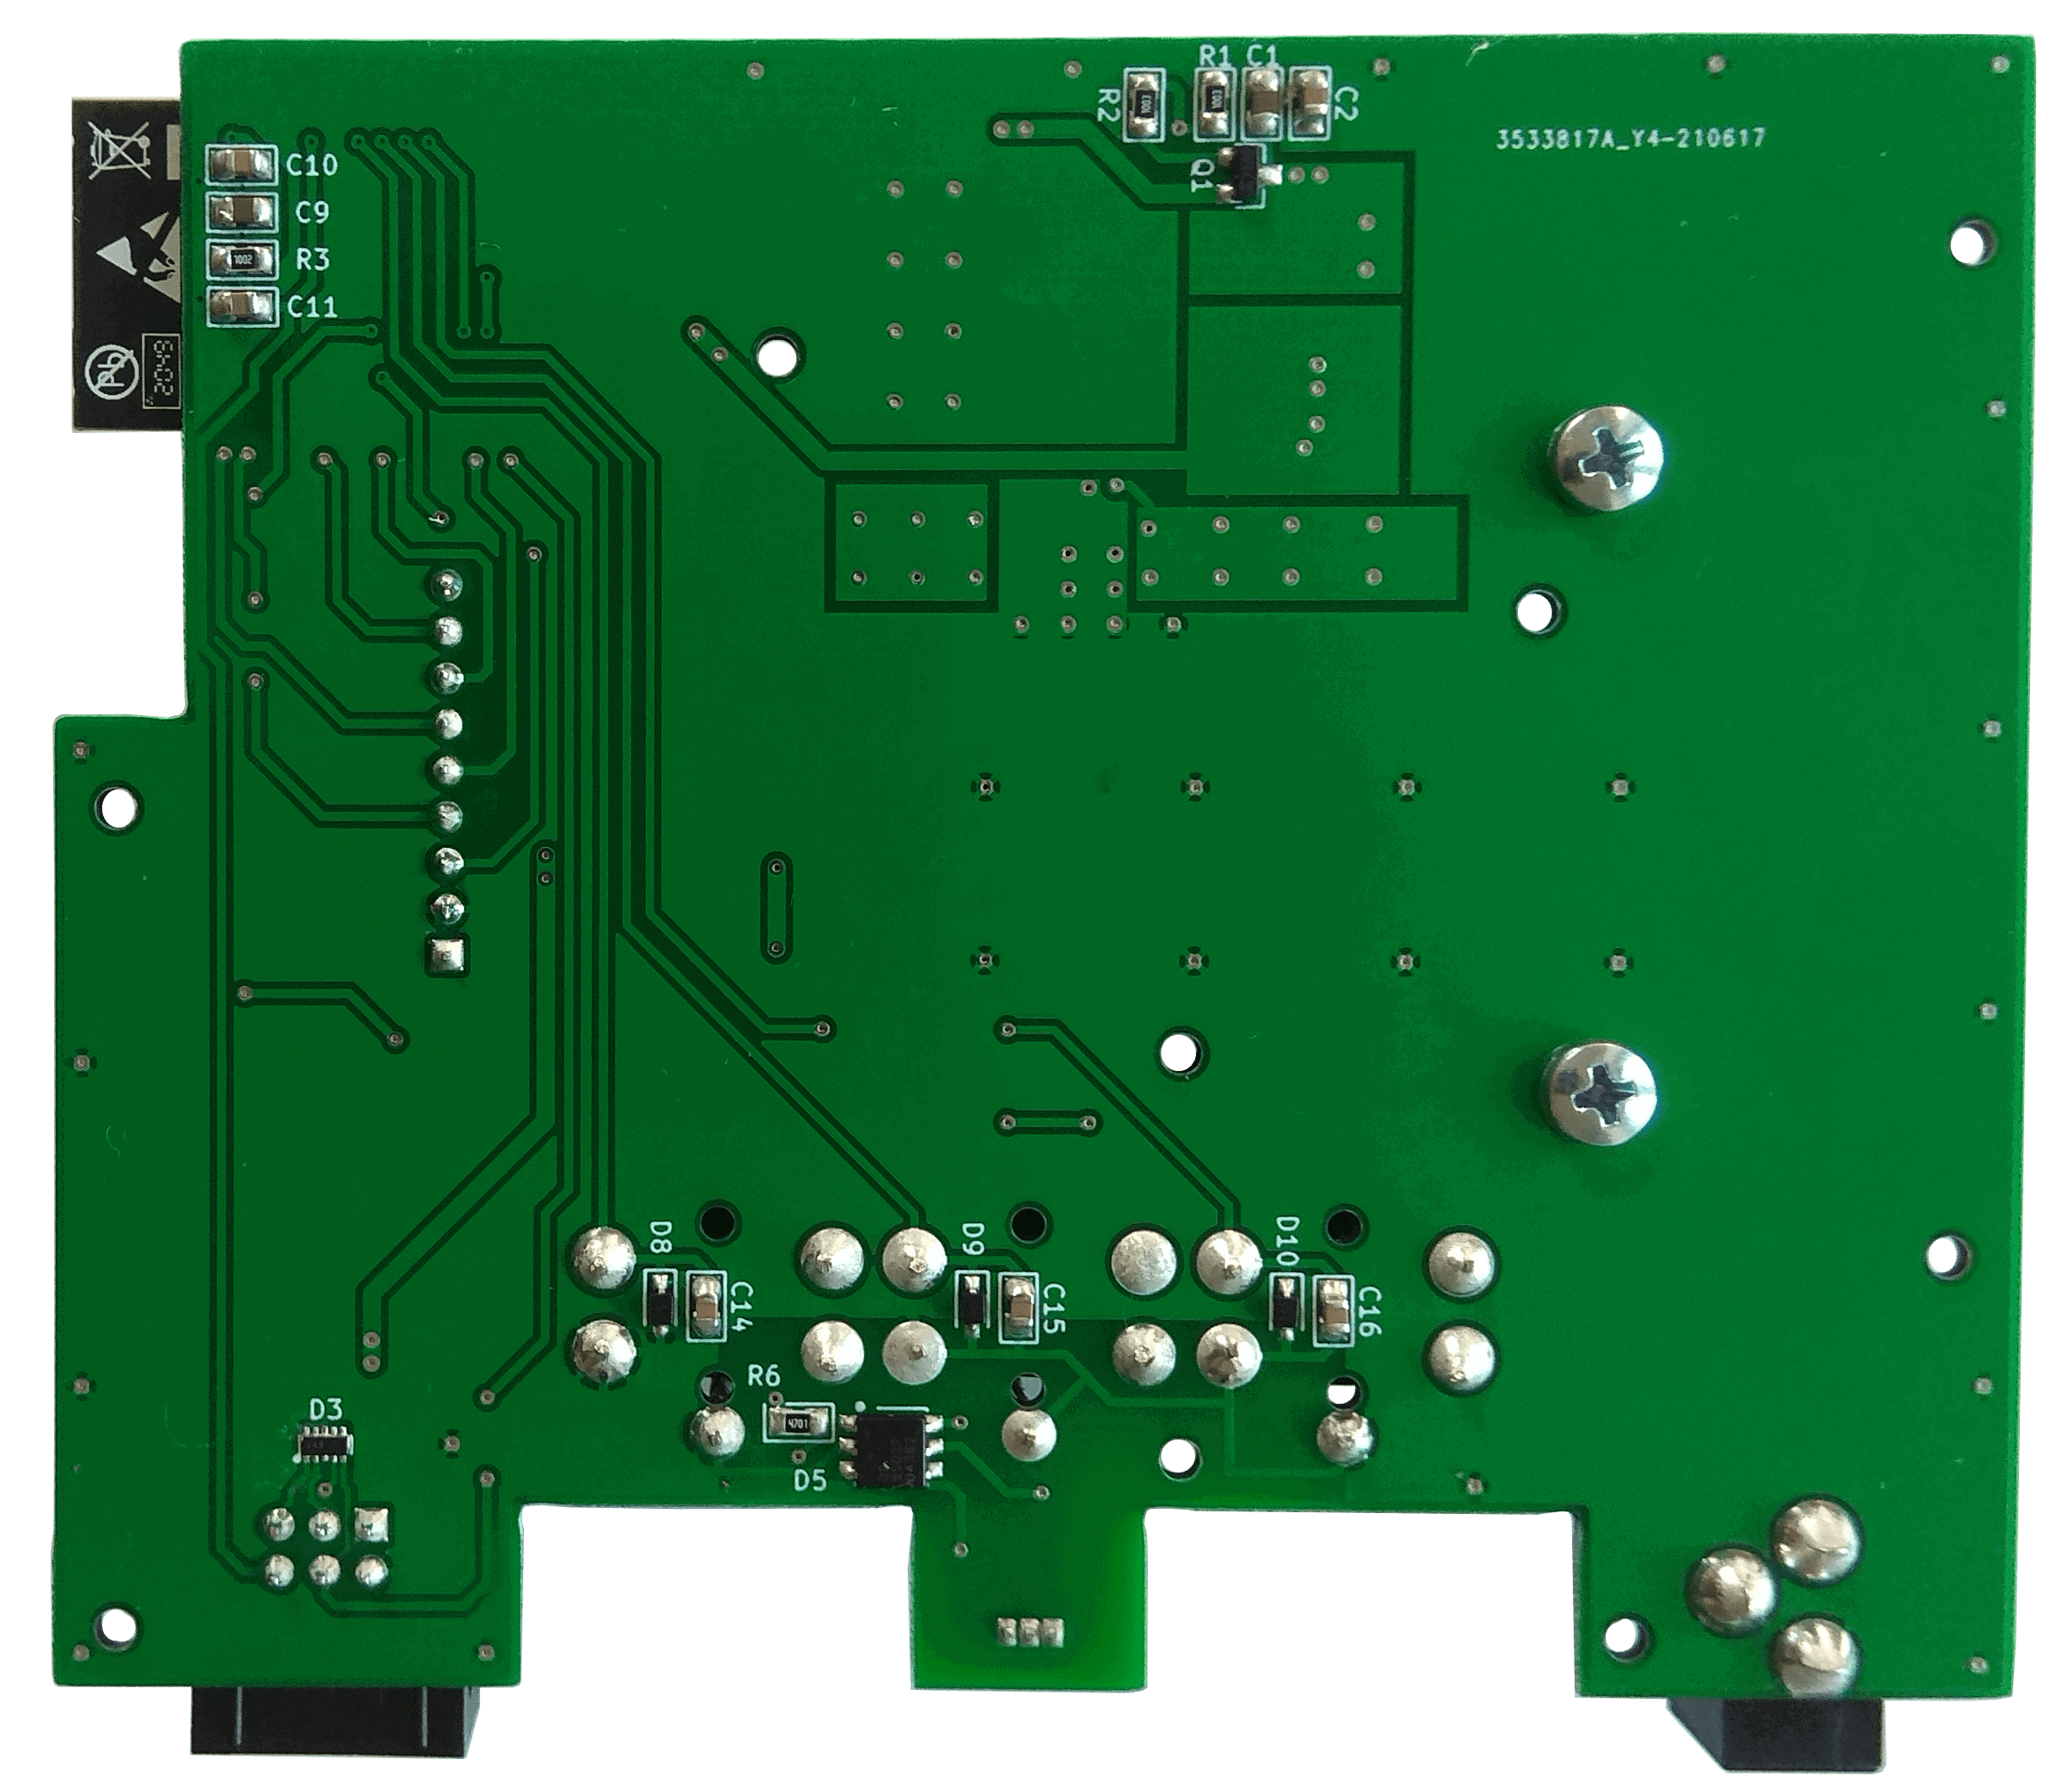
\includegraphics[width=\textwidth]{images/nastenny-snimac-prostorove-teploty-wifi/dps-nastenny-snimac-prostorove-teploty-wifi-spodni-cast.png}
    \caption{Spodní strana.}
    \label{fig:dps-nastenny-snimac-prostorove-teploty-wifi-spodni-cast}
\end{subfigure}
\caption{DPS nástěnného snímače prostorové teploty (verze WiFi).}
\label{fig:dps-nastenny-snimac-prostorove-teploty-wifi}
\end{figure}


\begin{figure}[H]
    \centering
    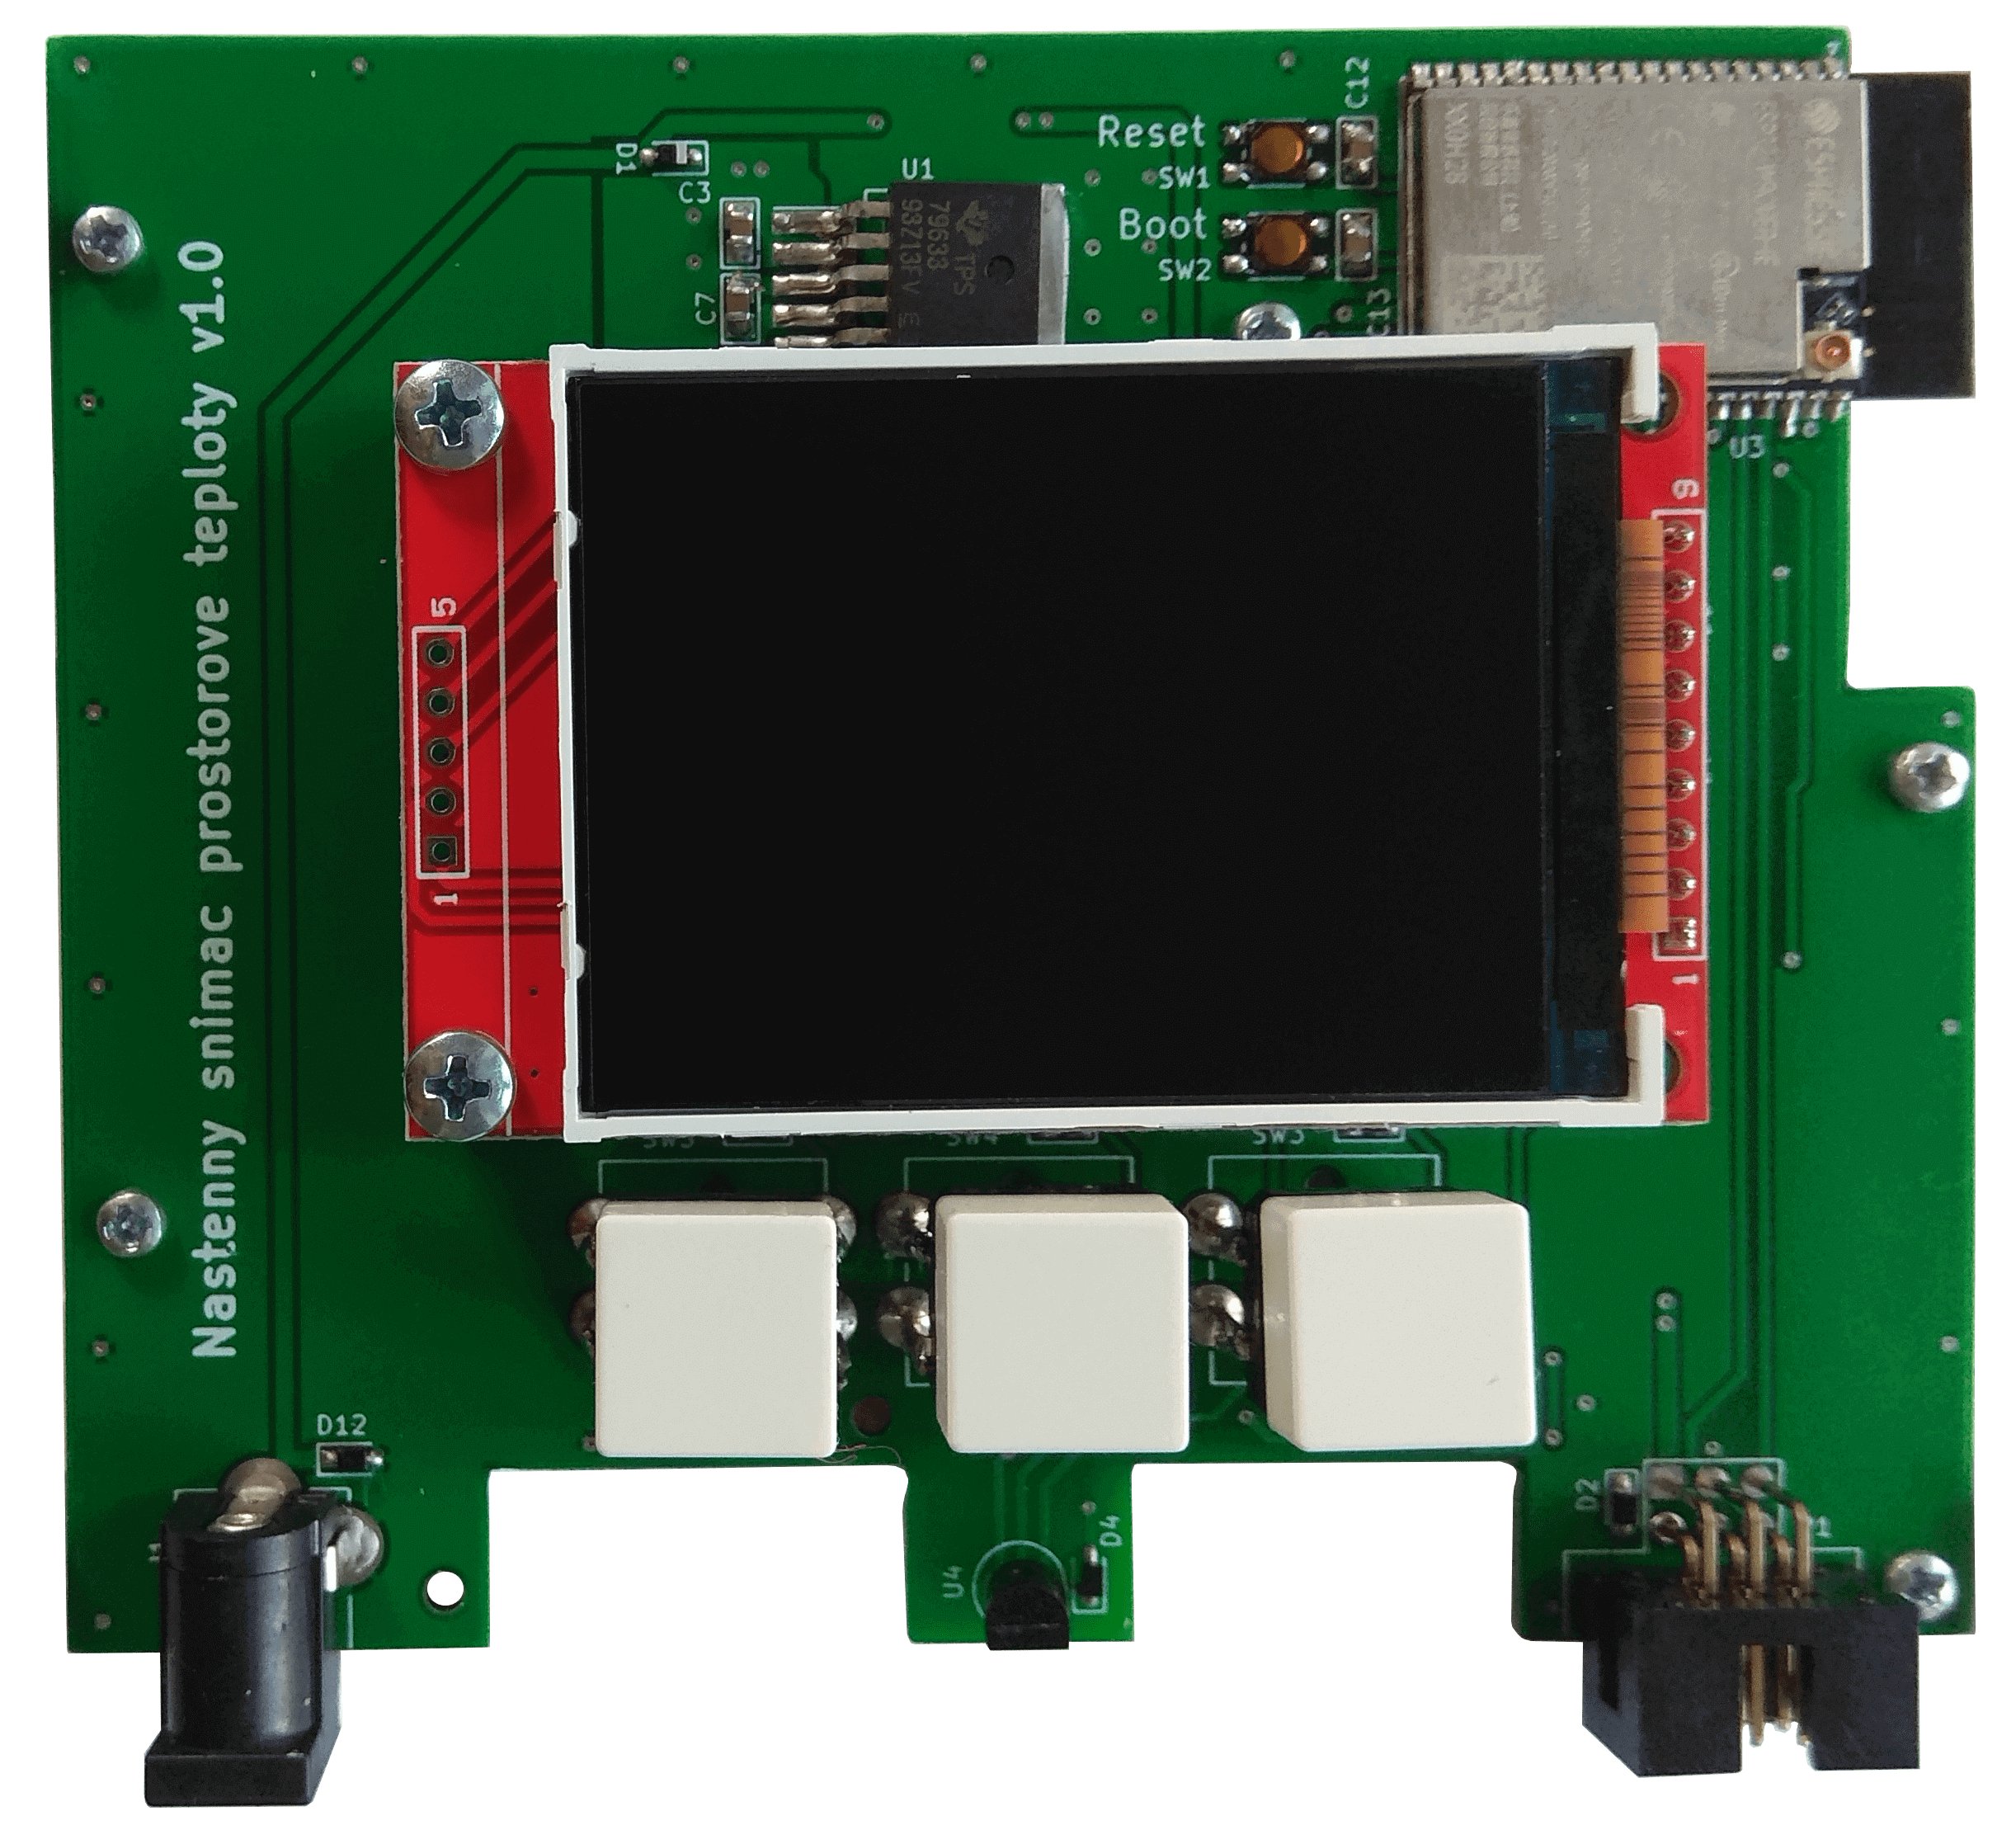
\includegraphics[width=0.85\textwidth]{images/nastenny-snimac-prostorove-teploty-wifi/dps-nastenny-snimac-prostorove-teploty-wifi-vrchni-cast-displej.png}
    \caption{DPS nástěnného snímače prostorové teploty (verze WiFi) s~displejem, vrchní strana.}
    \label{fig:dps-nastenny-snimac-prostorove-teploty-wifi-vrchni-cast-displej}
\end{figure}